\documentclass{article}[12pt]
\usepackage{physics}
\usepackage{setspace}
\usepackage{amsmath}
\usepackage{mathrsfs}
\usepackage{amssymb}
\usepackage{feynmp-auto}
\usepackage{tgtermes}
\usepackage{graphicx}
\usepackage{booktabs}
\usepackage{array}
\usepackage{caption}
\usepackage{listings}
\usepackage{xcolor}
\usepackage{helvet}
\definecolor{codegreen}{rgb}{0,0.6,0}
\definecolor{codegray}{rgb}{0.5,0.5,0.5}
\definecolor{codepurple}{rgb}{0.58,0,0.82}
\definecolor{backcolour}{rgb}{0.95,0.95,0.92}
\definecolor{lightgray}{rgb}{0.95,0.95,0.95}

\lstdefinestyle{mystyle}{
    backgroundcolor=\color{lightgray},   
    commentstyle=\color{codegreen},
    keywordstyle=\color{magenta},
    numberstyle=\tiny\color{codegray},
    stringstyle=\color{codepurple},
    basicstyle=\fontfamily{pcr}\selectfont\footnotesize,
    breakatwhitespace=false,         
    breaklines=true,                 
    captionpos=b,                    
    keepspaces=true,                 
    numbers=left,                    
    numbersep=5pt,                  
    showspaces=false,                
    showstringspaces=false,
    showtabs=false,                  
    tabsize=2
}
\setcounter{page}{23}
\lstset{style=mystyle}
\captionsetup{font=footnotesize}
\newcommand{\RN}[1]{%s
  \textup{\uppercase\expandafter{\romannumeral#1}}%
}
\usepackage{geometry}
\geometry{
 a4paper,
 left=25.4mm,
 right=25.4mm,
 top=30mm,
 bottom=25.4mm
 }
\begin{document}
\section*{5. Result}

\begin{spacing}{1.5}

\subsection*{single bath}

\begin{figure}[htbp]
  \centerline{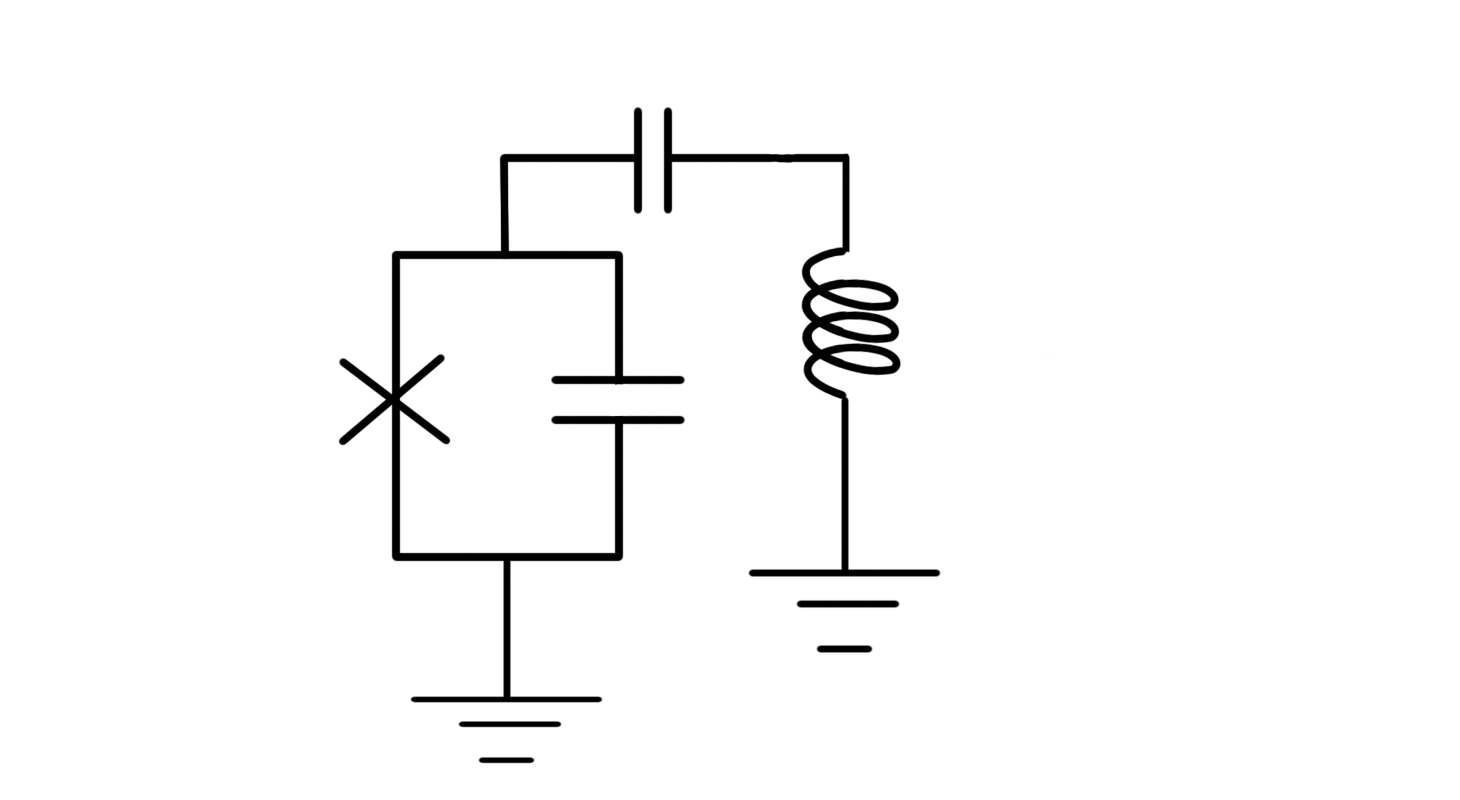
\includegraphics[width=10cm]{TexFigure/kps_singlebath.png}}
  \caption{Brief circuit scheme for single bath condition. The crossing symbol  refers to the insulated junction of Josephson junction.}
\end{figure}
First, we performed the benchmark test of the numerical program by comparing with the exact diagonalization (ED) method in the single mode (k=1) case.
\begin{figure}[htbp]
  \centerline{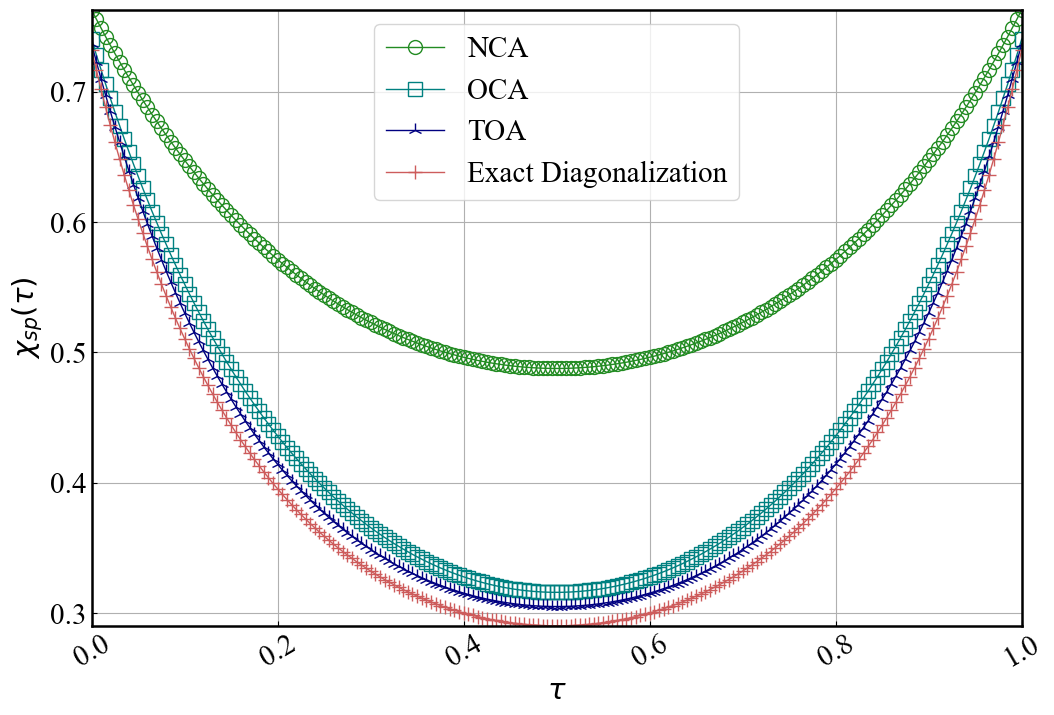
\includegraphics[width=10cm]{TexFigure/Res_bench_Fig1.png}}
  \caption{-edit-}
\end{figure}

\end{spacing}

\pagebreak
\newpage

\section*{ APPENDIX A. Perturbative field theory}
\begin{spacing}{1.5}
\subsection*{basic structure}

We can start our discussion in very basic perturbation field method which is adapting Wick’s theorem is available. To begin, we can define the partition function of configuration space that governed by the certain energy condition. The dynamic of variables of given space are governed under the action functional, thus partition function of space dictates the probability distribution of possible paths make system propagates onto. The partition function $Z[J]$ can be calculated in path integral method. For field $\phi(x,t)$ , corresponding Lagrangian is : 

\begin{flalign*}
\mathcal{L} =\frac{1}{2}\phi^TA\phi +\phi\cdot J \\ =\frac{1}{2}(-\phi^T \partial_t^2\phi + \phi^T \nabla^2\phi - m^2\phi) + J\phi
\end{flalign*}

Here, $A$ is a form of diagonal matrix. Consider only time in 4-vector notation, and use the above notation, we can write partition function in following:

\begin{flalign*}
Z[J]=\int[D\phi]e^{\int d\phi [\frac{1}{2}\partial^2_\tau\phi - m^2\phi^2]+J\cdot\phi}
\end{flalign*}

Which is, in short way:

\begin{flalign*}
Z[J]=Z[0]W[J]
\end{flalign*}

where $W[J]=e^{\frac{1}{2}J_iA^{-1}_{ij}J_j}$ , $Z[0] = \big(\frac{(2\pi i)^N}{\text{det}A}\big)^{\frac{1}{2}}$ . The sub indice $i,j$ means $i$th and $j$th element of $J(\phi)$. Based upon the probability distribution points of view, we can calculate the $n$th moment of the path distribution. In general, we can recognize that :

\begin{flalign*}
\langle \phi^{2n} \rangle = \frac{\int [D\phi] \phi^{2n} e^{\frac{1}{2} \phi^i A_{ij} \phi^j + J\cdot \phi}}{Z[0]} = \frac{\Pi_{i}\frac{ \mathcal{\delta}}{\mathcal{\delta}J_i}\frac{ \mathcal{\delta}}{\mathcal{\delta}J_j}\int[D\phi]e^{-\frac{1}{2}(J_{ij}A_{ij}J_{j})}}{Z[0]}= \Pi_{i}\frac{ \mathcal{\delta}}{\mathcal{\delta}J_i}\frac{ \mathcal{\delta}}{\mathcal{\delta}J_j} \ln{Z[J]}
\end{flalign*}

In general, this form of equation is constructed when exterior force or reaction caused to free propagating field. Now if there are some interaction happened between the field and the environment, especially in Lorentz-invariant action, we can treat its effect as a weak perturbation. Let $-\frac{g}{4}\phi^4$ is the perturbation term. Then the partition function turns out to be:

\begin{flalign*}
Z[J]=\int[D\phi]e^{\int d\phi [\frac{1}{2}\partial^2_\tau\phi - m^2\phi^2]+J\cdot\phi -\frac{g}{4}\phi^4}
\end{flalign*}

In same formula, we can write :

\subsection*{Perturbation theory and approximation method}

Guess if there are infinitesimal “real-time” variance appears in external Hamiltonian $H'$. We will treat it as a perturbation effect in the given Hamiltonian. In real-time procedure, let 

\begin{flalign*}
H'(t) = H'(t)+ \mathcal{\delta}H'(t)
\end{flalign*}

Using the above concept, We can rewrite the equation of motion for total Green’s function into : 

\begin{flalign*}
\{i \frac{\partial}{\partial t_1} +  \frac{\nabla^2_1}{2m} - H'(t_1) \pm \int dr_2 v(r_1-r_2)[G(t_1, t_1^+ ; H') + \frac{\mathcal{\delta}}{\mathcal{\delta} H'(t_1^+)}]\}G(t_1,t_1';H') = \mathcal{\delta} (t_1- t_1')
\end{flalign*}

Summarizing the result using local green’s function, we can get : 

\begin{flalign*}
G(t,t';H') =& G_0(t,t';H') \pm i \int^{-i\beta}_0 d\tau_1 d\tau_2 G_0(t,\tau_1;H')V(\tau_1-\tau_2) \\ 
&\bigg[G_0(\tau_2,\tau_2^+;H') + \frac{\mathcal{\delta}}{\mathcal{\delta} H'(\tau_2)}\bigg]G(\tau_1,t';H')
\end{flalign*}

This term can recursively solvable using the inverse matrix form of the bare Green’s function $G_0$,

\begin{flalign*}
G^{-1}(t,t';H') = \bigg[i\frac{\partial}{\partial t_1} + \frac{\nabla^2_1}{2m} - H(t)\bigg]\delta(t-t')
\end{flalign*}

And, 

\begin{flalign*}
\mathcal{\delta}G_0 = -G_0\mathcal{\delta}G_0^{-1}G_0
\end{flalign*}

Skipping the specific procedure, the final result of total Hamiltonian can be expanded to bare Green’s function with each time intervals : 

\begin{flalign*}
G(t,t';H') = G_0(t,t';H') \pm i\int^{-i\beta}_0 d\tau_1 d\tau_2 G_0(t,\tau_1;H')V(\tau_1-\tau_2)\bigg[G_0(\tau_2,\tau_2^+;H')G_0(\tau_1,t';H') \pm G_0(\tau_1,\tau_2^+;H')G_0(\tau_2;t_1;H')\bigg] 
\end{flalign*}

From the above derivation, we can get very basic two diagrams as and example of the result from the expansion. Corresponding diagrams are :

We can get more expanded term substitute the result recursively into $(***)$.

If we consider the interaction term with exterior conditions, we can use the concept of self-energy $\Sigma$ to describe the system’s dynamics. The self-energy $\Sigma$ is defined by : 

\begin{flalign*}
(i\frac{\partial}{\partial t_1} + H_0)G(t_1-t_1') - \int^{-i\beta}_0 d\tau_1 \Sigma(t_1-\tau_1)G(\tau_1-t_1) = \delta(t_1-t_1')
\end{flalign*}

And 

\begin{flalign*}
\Sigma(t,t';H')=\pm \int d\tau_2 V(t-\tau_2)G(\tau_2,\tau_2^+,H')\delta(t-t') + i \int d\tau_2 d\tau_1 V(t-\tau_2)\bigg[\frac{\delta G(t,\tau_1;H')}{\delta H'(\tau_2)}\bigg] G^{-1}(\tau,t',H')
\end{flalign*}

Which can be compare with the equation $(*)$ , form of the equation brings out full Green’s function G,
\end{spacing}

\end{document}